\documentclass[11pt]{article}

% --- Packages ---
\usepackage[margin=1in]{geometry}
\usepackage{amsmath,amssymb}
\usepackage{graphicx}
\usepackage{booktabs}
\usepackage{array}
\usepackage{hyperref}
\usepackage{xurl}
\usepackage{authblk}
\usepackage{orcidlink}
\usepackage{xcolor}
\usepackage{caption}
\usepackage{subcaption}
\usepackage{enumitem}
\usepackage{microtype}
\setlength{\emergencystretch}{3em}
\usepackage[T1]{fontenc}
\usepackage{lmodern}

% --- Hyperref setup ---
\hypersetup{
  colorlinks=true,
  linkcolor=blue!70!black,
  citecolor=blue!70!black,
  urlcolor=blue!60!black,
}

% --- Title ---
\title{FairDerm: Evaluating the Limits of Photometric Augmentation for Skin-Tone Bias in Melanoma Detection}

\author[1,*]{Shanmuka Gottimukkala \orcidlink{0009-0002-2991-1249}}
\author[2]{Dr. Vaibhav C. Gandhi \orcidlink{0000-0001-8454-3093}}
\affil[1]{Milton High School, 13025 Birmingham Highway, Milton, GA 30004, USA}
\affil[2]{Department of Computer Engineering, Madhuben and Bhanubhai Patel Institute of Technology (MBIT), The Charutar Vidya Mandal (CVM) University, Gujarat, India}
\affil[*]{Corresponding author: only.shan@outlook.com}

\date{September 2026}

\begin{document}

\maketitle

% --- Abstract ---
\begin{abstract}
\textbf{Background:} Dermatological deep learning models have been shown to exhibit performance disparities across skin tones, with diagnostic accuracy often degrading substantially for darker skin presentations \cite{Daneshjou2022}. Such biases threaten the equitable deployment of clinical decision support tools and may exacerbate existing health disparities in dermatology.

\textbf{Methods:} We evaluate melanoma classification bias on the Dermatology Data Initiative (DDI) dataset \cite{DDI2021}, which provides skin-tone annotations \cite{Fitzpatrick1988} enabling subgroup analysis. An EfficientNet-B0 model is pretrained on HAM10000 and fine-tuned on DDI. We then apply targeted augmentation using saved photometric and geometric transforms (color jitter, noise, elastic deformation, rotations; no generative model), with augmentation factors of 0$\times$, 2$\times$, 5$\times$, and 10$\times$, drawing images round-robin across all 29 source lesions at every factor. Stages 2 and 3 share learning rate, batch size, frozen layers, and epoch budget. Because augmentation changes the effective class ratio, we additionally re-run Stage 3 from a common checkpoint under three class-weighting regimes to separate the augmentation effect from the imbalance shift, and we repeat the full pipeline across 5 seeds. Generated images derive exclusively from training-split dark-skin melanomas ($n\,{=}\,29$, 10 variants each, 290 total), and their provenance is verified per image rather than assumed. Bootstrap 95\% confidence intervals (1{,}000 iterations) are reported throughout.

\textbf{Results:} The pretrained baseline achieved overall AUROC 0.662 and Dark subgroup AUROC 0.588. Fine-tuning produced overall AUROC 0.634 and Dark AUROC 0.547, while adding 290 train-only generated dark melanomas produced overall AUROC 0.639 and Dark AUROC 0.481 (seed-42 split). The paired Dark AUROC delta for augmentation was $-0.066$ (95\% bootstrap interval $[-0.151,0.008]$, $p\,{=}\,0.962$; one-tailed directional, $H_1$: Dark improvement $>0$, $p$\,$=$\,proportion of bootstrap $\Delta \leq 0$). Once ablation arms are matched on frozen layers and lesion coverage, generated-image quantity has no measurable effect on Dark AUROC (0.509, 0.513, 0.503, 0.497 at 0$\times$, 2$\times$, 5$\times$, 10$\times$) and reduces Light AUROC across the range tested (0.784 to 0.697, with a small 2$\times$-to-5$\times$ fluctuation). Holding the fine-tuned checkpoint fixed and varying only the class-weighting regime gave Dark AUROC 0.484 (pre-augmentation \texttt{pos\_weight} 2.853), 0.478 (recomputed \texttt{pos\_weight} 0.742, same images), and 0.550 (balanced composition and \texttt{pos\_weight} 1.0 with 101 generated dark benign images added), narrowing the Light--Dark gap from $-0.222$ to $-0.141$. Because single-split estimates proved unstable, we repeated the entire pipeline across five seeds (42--46), re-deriving the split, generated images, and class ratio per seed: mean Dark AUROC was $0.575 \pm 0.145$ fine-tuned versus $0.604 \pm 0.152$ with generated images, a paired Dark AUROC delta of $+0.028$ (seed-level 95\% interval $[-0.001, 0.057]$, not significant), and the Dark$-$Light gap was unchanged ($-0.081 \pm 0.193$ versus $-0.083 \pm 0.161$). Between-seed variability exceeds every between-stage difference, and the gap sign flips across seeds, so the seed-42 point estimates (Dark AUROC 0.547 to 0.481) should be read as one draw from a high-variance distribution rather than as an effect size.

\textbf{Conclusions:} Across five seeds (primary), heuristic photometric augmentation from a small source pool left the skin-tone performance gap unchanged and produced no statistically significant Dark AUROC change (delta $+0.028$, 95\% seed-level CI $[-0.001,0.057]$). The seed-42 single-split result is one draw from a high-variance distribution and the gap sign flips across seeds. The degradation in the headline configuration is substantially attributable to the class-composition and weighting confound quantified by the arm study. All experiments are DDI-only ($n=656$); no external validation on Fitzpatrick17k, HAM10000 test, or clinical cohorts, so generalizability is not demonstrated. With low power (Dark test subgroup $\sim$10 melanomas per seed) and limited augmentation diversity, these findings are best interpreted as a \emph{negative/methodology evaluation study} rather than evidence of an AI improvement. Multi-centre cohorts, independent validation, clinician review of generated-image realism, and diversity metrics are needed.
\end{abstract}

\vspace{0.5em}
\noindent\textbf{Keywords:} Algorithmic Fairness, Dermatology AI, Melanoma Classification, Data Augmentation, EfficientNet, Skin-Tone Bias


% --- Body ---
\section{Introduction}

Deep learning models for skin lesion classification have achieved dermatologist-level accuracy on curated benchmarks, yet their performance is not uniform across skin tones. Systematic evaluations have revealed that diagnostic models trained predominantly on lighter skin tones exhibit degraded sensitivity and specificity on darker skin presentations \cite{Esteva2017, Daneshjou2022}. Groh et al.~\cite{Groh2021} documented substantial variation in model performance across Fitzpatrick skin types, underscoring that reported aggregate metrics can mask critical disparities. These findings raise concerns about the equitable clinical deployment of dermatological AI, particularly for populations that already face barriers to dermatologic care \cite{Adamson2018}.

The Dermatology Data Initiative (DDI) dataset represents a recent effort to address this gap by providing diverse clinical images with skin-tone annotations \cite{DDI2021}, interpreted using the Fitzpatrick scale \cite{Fitzpatrick1988}. However, the dataset remains small relative to large-scale benchmarks, and dark-skin melanoma cases are particularly scarce. The HAM10000 dataset \cite{Tschandl2018}, while substantially larger, lacks skin type annotations and skews toward lighter skin presentations. This class imbalance means that models pretrained on such data may encode skin-tone priors that propagate into downstream fine-tuning, especially when dark-skin melanoma examples number fewer than 50.

Data augmentation offers a practical approach to mitigating training-set imbalance without requiring additional clinical data collection. Modern augmentation libraries such as Albumentations \cite{Buslaev2020} support principled color-space and geometric perturbations that can expand the effective diversity of underrepresented subgroups. Fairness-aware augmentation strategies have been explored in general machine learning contexts \cite{Mehrabi2021}, though their application to dermatological classification remains under-studied.

In this work, we investigate targeted augmentation as a fairness intervention for melanoma detection across skin tones on the DDI dataset. Our contributions are fivefold: (1) we quantify the skin-tone bias gap in an EfficientNet-B0 model pretrained on HAM10000 and fine-tuned on DDI, revealing near-chance performance on dark-skin melanoma; (2) we evaluate a train-only augmentation pipeline ($n\,{=}\,29$ source dark melanomas, 290 generated images) and show that simple photometric transforms do not improve Dark AUROC ($0.547 \to 0.481$, paired $\Delta\,{=}\,-0.066$, $p\,{=}\,0.962$), demonstrating the limits of color-jitter fairness interventions; (3) we measure a confounder that this design introduces but that the headline number alone cannot reveal, by holding the fine-tuned checkpoint fixed and varying only the class weighting and generated-image composition, and find that balancing the composition recovers Dark AUROC to 0.550 and narrows the Light--Dark gap from $-0.222$ to $-0.141$; (4) we report per-image provenance for all 290 generated images by hash and perceptual descriptor rather than asserting it; and (5) we repeat the full pipeline over 5 seeds so that reported effects carry a standard deviation rather than a single run. Main results are summarized in Table~\ref{tab:main_results}, with detailed subgroup AUROC values in Table~\ref{tab:subgroup_auroc} and visualized in Figure~\ref{fig:subgroup_auroc}.

\section{Methods}

\subsection{Dataset}

We use two dermatoscopic image datasets. The HAM10000 dataset \cite{Tschandl2018} contains 10,015 dermatoscopic images from diverse populations, annotated with seven diagnostic categories. For binary melanoma classification, we retain only melanocytic lesions: 7,818 samples comprising melanoma (\emph{mel}) and melanocytic nevus (\emph{nv}) classes, yielding a malignant--benign ratio of approximately 14:86. No skin tone labels are available in HAM10000.

The Dermatology Data Initiative (DDI) dataset provides 656 dermatoscopic images with diverse skin-tone annotations \cite{DDI2021}. We interpret its numeric skin-tone codes using the Fitzpatrick scale \cite{Fitzpatrick1988}: 12 (Light, Fitzpatrick I--II), 34 (Medium, Fitzpatrick III--IV), or 56 (Dark, Fitzpatrick V--VI). All three subgroups are evaluated; the Medium subgroup is reported as a secondary analysis because its smaller melanoma count makes its estimates less stable than the Light and Dark subgroups.

DDI is split into train/validation/test partitions using a 60/20/20 ratio, stratified by the cross-product of label $\times$ skin tone to preserve class balance across subgroups. The split is saved for reproducibility (see Appendix). The resulting partition sizes are: Train\,$=$\,393, Validation\,$=$\,131, Test\,$=$\,132. The test set contains 42 Light samples (10 melanoma), 48 Medium samples (8 melanoma), and 42 Dark samples (10 melanoma). \emph{Power note:} The Dark test subgroup contains $n=42$ images with only $\sim 10$ melanoma cases, yielding large bootstrap uncertainty (bootstrap SD $\sim 0.15$ AUROC and 95\% CI half-width $\sim 0.20$; see Table~\ref{tab:subgroup_auroc}). Single-split fairness comparisons are fragile by construction; between-seed variability (SD $\approx 0.145$--$0.152$ for Dark AUROC) exceeds all between-stage differences (paired delta $\approx +0.028$). Accordingly, 5-seed aggregation is primary and seed-42 is treated as one draw from a high-variance distribution. All experiments use the DDI dataset only ($n=656$) for fine-tuning and evaluation. No external validation is performed on independent datasets (e.g., Fitzpatrick17k, HAM10000 held-out test sets, or clinical multi-centre cohorts); generalizability has not been demonstrated and requires future work. Split disjointness is enforced via assertion checks on filenames, and a byte-level SHA256 overlap check confirms that no generated image shares bytes with any held-out image. Dataset composition is summarized in Table~\ref{tab:dataset}.

\subsection{Model Architecture}

We use EfficientNet-B0 \cite{Tan2019EfficientNet} as the backbone architecture, with the final classifier layer replaced by a single-output linear layer for binary melanoma classification. The full model contains 4,008,829 parameters. Weights are initialized from ImageNet pretraining. Input images are resized to $224 \times 224$ and normalized with ImageNet channel statistics (mean $[0.485, 0.456, 0.406]$, std $[0.229, 0.224, 0.225]$).

Transfer learning follows a partial-freezing strategy. During the fine-tuning and generated-augmentation stages, early convolutional feature extractor layers are frozen, and only the final two feature blocks (\texttt{features.6}, \texttt{features.7}) and the classifier head are trained, leaving 2,744,861 trainable parameters. This reduces the number of trainable parameters relative to full fine-tuning while allowing the model to adapt high-level representations to the target domain. The generated-image ablation study uses this identical frozen-layer configuration, so its arms differ only in the number of generated images.

\subsection{Training Pipeline}

The pipeline consists of three sequential stages, each initializing from the preceding stage's checkpoint. Stage 1 uses its own hyperparameters as a pretrained initialization; Stages 2 and 3 share learning rate, weight decay, batch size, frozen-layer configuration, and epoch budget, so the only intended difference between them is the addition of generated images. We report the one remaining difference---the epoch budget of the ablation arms---explicitly rather than describing the comparison as fully controlled. Hyperparameters are summarized in Table~\ref{tab:training_config}.

\paragraph{Stage 1: Baseline.}
The model is trained on the full HAM10000 mel/nv subset (80/20 stratified split) for up to 10 epochs with early stopping (patience\,$=$\,3). The binary cross-entropy loss \texttt{BCEWithLogitsLoss} is used with no class weighting. The optimizer is AdamW with learning rate $3 \times 10^{-4}$ and weight decay $10^{-4}$. A \texttt{ReduceLROnPlateau} scheduler (factor\,$=$\,0.5, patience\,$=$\,2) monitors validation AUROC. This stage uses different hyperparameters from Stages 2--3, which is acceptable as it serves only as a pretrained initialization.

\paragraph{Stage 2: Fine-tuning.}
The baseline checkpoint is loaded, feature extractor layers are frozen as described above, and the model is fine-tuned on the DDI training partition for up to 10 epochs with early stopping (patience\,$=$\,3). The malignant--benign class imbalance in DDI is addressed by computing \texttt{pos\_weight} dynamically from the training split as $n_{\text{neg}} / n_{\text{pos}}$. The optimizer is AdamW with learning rate $5 \times 10^{-5}$ and weight decay $10^{-4}$, applied only to unfrozen parameters. Batch size is 32.

\paragraph{Stage 3: Generated Augmentation.}
The fine-tuned checkpoint is loaded with the same frozen-layer configuration. The DDI training set is augmented with generated dark-skin melanoma images (described in Section~\ref{sec:synthetic_aug}) and trained for up to 10 epochs (patience\,$=$\,3). Learning rate $5 \times 10^{-5}$, weight decay $10^{-4}$, batch size 32, and early-stopping patience are identical to Stage 2.

\textbf{Stage 3 confound note:} Generating only dark-skin melanomas (29$\to$290) while keeping \texttt{pos\_weight}$= n_{\text{neg}}/n_{\text{pos}}$ computed on the pre-augmentation training split ($291/102=2.8529$) changes the combined training class ratio from 102/291 (pos/neg) to 392/291; the balanced ratio for the combined set is $291/392=0.7423$. This over-weights malignancy in the augmented dark-skin portion by a factor of $\approx 3.8\times$ relative to the true combined distribution. Consequently, the headline Stage 2$\to$3 contrast does \emph{not} isolate the effect of augmentation alone; attribution is confounded by class composition and weighting. We quantify this via the arm study (Section~\ref{sec:pw\_arms}).

\paragraph{Class-imbalance weighting and the Stage~2/Stage~3 contrast.}
The \texttt{pos\_weight} applied in Stage 3 is the Stage-2 value $n_{\text{neg}} / n_{\text{pos}} = 291 / 102 = 2.8529$, computed on the pre-augmentation training split. Adding 290 generated images raises the effective positive count to 392 against 291 negatives, so the balanced ratio for the set actually presented to the loss is $291/392 = 0.7423$. The retained weighting therefore over-weights the minority class relative to the augmented set by a factor of $\approx 3.8$. This is not an incidental detail: it is a class-imbalance change that accompanies the augmentation, and it confounds attribution of any Stage~2 to Stage~3 difference to the generated images alone. We report it explicitly rather than describing the contrast as a clean single-variable comparison, and Section~\ref{sec:pw_arms} isolates its effect by re-running Stage 3 under three weighting regimes from the same Stage-2 checkpoint. The headline result in Section~\ref{sec:results} is the pre-existing configuration, and we note it is not the configuration that isolates the intended effect.

\paragraph{Hyperparameter standardization.}
Stages 2 and 3 share learning rate, weight decay, batch size, frozen layers, and epoch budget, and differ in the added generated images and in the implied class ratio discussed above. The ablation arms (Section~\ref{sec:ablation}) hold all Stage-3 hyperparameters fixed and vary only the number of generated images. Stage 1 differs in learning rate and batch size but serves only as a pretrained initialization.

\subsection{Generated-Image Augmentation}
\label{sec:synthetic_aug}

Our generated images are \emph{saved photometric and geometric transforms}, not samples from a generative model: we use the Albumentations library \cite{Buslaev2020} to apply fixed random transforms to existing training lesions, so no GAN or diffusion model is involved. From the dark-skin melanoma examples in the DDI \emph{training split} ($n\,{=}\,29$), each source image is transformed 10 times, yielding 290 generated images. We refer to these as \emph{generated} rather than \emph{synthetic} throughout, to avoid implying a generative model. Generated images derive exclusively from training-split data and never from validation or test images.

Because these are transformed copies of individual lesions rather than independent samples, we verified their provenance rather than assuming it. For each of the 290 generated images we computed a 32-dimensional descriptor and searched for its nearest neighbour among DDI images under all 8 dihedral transforms; the 32 darkest principal components were used to suppress colour and intensity, which dominate raw-pixel distances. All 290 images matched a \emph{training}-split dark melanoma as the nearest neighbour, none matched a held-out image, and all 29 source lesions were exercised. Median similarity to the matched training source was 0.9985 and the median margin over the best held-out decoy was $+0.2706$ (minimum margin $+0.0766$). Exact-duplicate exclusion is handled separately by a byte-level SHA256 check. The full per-image provenance report is provided in the Appendix.

The augmentation pipeline applies the following transforms in sequence:
\begin{enumerate}
    \item \textbf{RandomBrightnessContrast}: brightness and contrast variation ($\pm 0.2$ range, probability\,$=$\,0.8)
    \item \textbf{HueSaturationValue}: hue shift ($\pm 10$), saturation shift ($\pm 20$), value shift ($\pm 15$), probability\,$=$\,0.7
    \item \textbf{GaussNoise}: additive Gaussian noise, probability\,$=$\,0.2
    \item \textbf{ElasticTransform}: smooth geometric deformation ($\alpha\,{=}\,0.5$, $\sigma\,{=}\,5$), probability\,$=$\,0.1
    \item \textbf{RandomRotate90}: 90$^\circ$ rotation multiples, probability\,$=$\,0.5
    \item \textbf{HorizontalFlip}: mirror reflection, probability\,$=$\,0.5
\end{enumerate}

All outputs are resized to $224 \times 224$ and saved as JPEG files. Generated images are added to the DDI training set via \texttt{ConcatDataset}, increasing the effective training size from 393 to 683 samples. They are never added to validation or test partitions. The transform pipeline is seeded, so the generated set is reproducible for a given seed. Split disjointness and byte-level SHA256 overlap with held-out images are verified as described in the Appendix.

\textbf{Augmentation diversity (limitation):} The 290 generated images are photometric and geometric transforms of only 29 source lesions (10 variants each). No FID score is computed, no clinician review of lesion preservation was performed, and no comparison to generative models (e.g., diffusion/GAN) is made. Provenance checks show median descriptor similarity 0.9985 to the matched training source (confirming near-duplicates of the originals), with the minimum margin over the best held-out decoy $+0.0766$ and byte-level SHA256 excluding exact duplicates. Thus diversity is bounded by the source distribution.

\subsection{Class-Imbalance Arm Study}
\label{sec:pw_arms}

To separate the effect of augmentation from the accompanying change in class ratio, we re-run Stage 3 from the \emph{same} Stage-2 checkpoint under three arms that differ only in \texttt{pos\_weight} and generated-image composition. All arms share seed, split, frozen layers, learning rate, weight decay, batch size, and epoch budget.

\begin{itemize}
    \item \textbf{static}: \texttt{pos\_weight} $= 2.8529$ (the pre-augmentation ratio), 290 dark-melanoma generated images. This is the configuration underlying the headline result.
    \item \textbf{recomputed}: \texttt{pos\_weight} $= 0.7423$, the ratio of the actual combined set, with the same 290 generated images. This isolates the weighting change from any change in generated volume.
    \item \textbf{symmetric}: 101 dark-benign generated images added (spread over the 95 dark benign training lesions) so the combined set is exactly balanced at 392 positives and 392 negatives, with \texttt{pos\_weight} $= 1.0$. Here augmentation changes neither the class ratio nor the loss weighting.
\end{itemize}

This design isolates how much of the Stage-2 to Stage-3 change is attributable to the generated images rather than to the reweighting they induce.

\subsection{Evaluation}

The primary metric is the Area Under the Receiver Operating Characteristic curve (AUROC) \cite{Hanley1982}, which is threshold-independent and thus suitable for comparing models at different operating points. Secondary threshold-dependent metrics---sensitivity, specificity, positive predictive value (PPV), and F1 score---are also reported.

Classification thresholds for all three DDI test evaluations use Youden's $J$ statistic (maximizing $\text{TPR} - \text{FPR}$) computed on the corresponding validation predictions. AUROC is the primary evaluation metric as it is threshold-independent and appropriate for cross-stage comparison. Sensitivity, specificity, PPV, and F1 are threshold-dependent and computed using per-stage Youden's $J$ thresholds optimized on the corresponding validation set; as such, they are not directly comparable across stages. No matched-threshold analysis (fixed operating point across stages) was performed. For example, Light versus Dark sensitivity values reflect different operating points chosen per stage/validation split. The tables that report threshold-dependent metrics carry a note to that effect.

For uncertainty quantification, bootstrap 95\% confidence intervals are computed using 1{,}000 resampling iterations with the percentile method \cite{Efron1986}. Iterations that produce degenerate samples (single-class bootstrap draws) are discarded. Bootstrap analysis uses a fixed random seed (seed\,$=$\,0) for the random number generator. A permutation-based p-value is computed for the Dark AUROC improvement between Stages 2 and 3: the proportion of bootstrap AUROC differences $\leq 0$ across 1{,}000 paired resamples.

Subgroup analysis stratifies predictions by Fitzpatrick skin type code: Light (code 12, Fitzpatrick I--II), Medium (code 34, Fitzpatrick III--IV), and Dark (code 56, Fitzpatrick V--VI). All three are reported. Because the test set contains 8 melanomas in the Medium subgroup versus 10 in each of Light and Dark, Medium estimates carry wider uncertainty and are interpreted as secondary. Given the small subgroup sizes ($n\,{=}\,42$--$48$, 8--10 melanomas), all subgroup conclusions should be treated as preliminary and directional.

\subsection{Five-Seed Robustness}

Single-split results on 132 test images can move substantially under resampling, so we repeat the entire three-stage pipeline across 5 seeds (42--46). For each seed we regenerate the stratified DDI split, retrain the Stage-1 HAM10000 baseline, retrain Stages 2 and 3, regenerate the 290 generated images with that seed's transform seed, and re-derive all metrics on that seed's test set. We report the mean, sample standard deviation (ddof\,$=$\,1), and a seed-level percentile bootstrap 95\% confidence interval over the 5 seeds for each reported quantity. The Stage-1 baseline is retrained per seed rather than reused, so the reported variation reflects the full pipeline.

\section{Experiments}

\subsection{Experimental Setup}

All experiments were conducted on an Apple Silicon Mac (MPS backend) using PyTorch 2.8.0, torchvision 0.23.0, and NumPy 2.0.2. Python, NumPy, and PyTorch random number generators were seeded, and the image-augmentation pipeline is seeded, so the generated image set is reproducible for a given seed. The headline analysis uses seed 42; Section~\ref{sec:multiseed_results} reports a separate 5-seed replication. Due to floating-point non-determinism in the MPS backend, exact numerical reproduction on different hardware is not guaranteed.

Stages 2 and 3 share learning rate $5{\times}10^{-5}$, batch size 32, weight decay $10^{-4}$, frozen-layer configuration, and a 10-epoch budget. Stage 1 uses a larger batch size and a higher learning rate, as it serves only as a pretrained initialization. Stage 3 additionally differs from Stage 2 in the class ratio implied by the added images, which we treat as an explicit experimental factor rather than a controlled constant (Sections~\ref{sec:synthetic_aug} and \ref{sec:pw_arms}).

\subsection{Baseline}

The baseline model is trained exclusively on HAM10000 (7{,}818 mel/nv samples) with an 80/20 stratified split. No DDI data is used at this stage. The model used the documented 10-epoch limit with early stopping, and was selected on HAM10000 validation AUROC.

\subsection{Fine-tuning}

The baseline is fine-tuned on the DDI training split (393 samples) with early feature blocks frozen. The fine-tuned checkpoint is the initialization for Stage 3 and for the class-imbalance arm study, so all three Stage-3 arms in Section~\ref{sec:pw_arms} share it exactly.

\subsection{Generated Augmentation}

Stage 3 adds 290 generated dark-skin melanoma images, drawn exclusively from the 29 training-split dark melanomas, as described in Section~\ref{sec:synthetic_aug}. Provenance is verified per image rather than assumed: byte-level SHA256 confirms no held-out bytes are duplicated, and a dihedral-invariant perceptual check confirms every generated image matches a training source rather than a held-out one.

\subsection{Ablation Study}

We ablate over the number of generated images, testing multipliers of 0$\times$ (none), 2$\times$ (58 images), 5$\times$ (145 images), and 10$\times$ (290 images). Images are selected round-robin across all 29 source lesions, so each multiplier adds variants of every lesion instead of concentrating on the first few; this makes the arms differ in quantity rather than in lesion identity. All arms start from the fine-tuned checkpoint, freeze the same layers as Stage 3, and share Stage-3 learning rate, weight decay, batch size, and \texttt{pos\_weight}. They use a 5-epoch budget rather than Stage 3's 10, so the 10$\times$ arm is not a fully matched replica of the headline run; this is stated in the results rather than glossed over.

\subsection{Class-Imbalance Arm Study}

Section~\ref{sec:pw_arms} defines three Stage-3 arms that share the fine-tuned checkpoint and differ only in \texttt{pos\_weight} and generated-image composition. The ablation varies quantity at a fixed weighting; this study varies the weighting at fixed checkpoint. Together they separate the two factors that the headline configuration changes simultaneously.

\subsection{Multi-Seed Replication}

The 5-seed study regenerates the stratified DDI split, retrains all three stages, regenerates the 290 images with that seed's transform seed, and re-derives all metrics on that seed's test set. The Stage-1 baseline is retrained per seed so the reported standard deviation reflects the full pipeline rather than one fixed initialization.

\section{Results}
\label{sec:results}

\subsection{Main Results}

Table~\ref{tab:main_results} presents the primary classification performance across three model stages: a pretrained baseline, a fine-tuned model, and a fine-tuned model augmented with 290 generated dermoscopy images. Stages 2 and 3 share learning rate, weight decay, batch size, frozen layers, and epoch budget. The augmentation is additionally accompanied by a change in effective class ratio, which we quantify separately in Section~\ref{sec:pw_arms_results} rather than attributing the whole Stage-2 to Stage-3 difference to the generated images.

\begin{figure}[htbp]
  \centering
  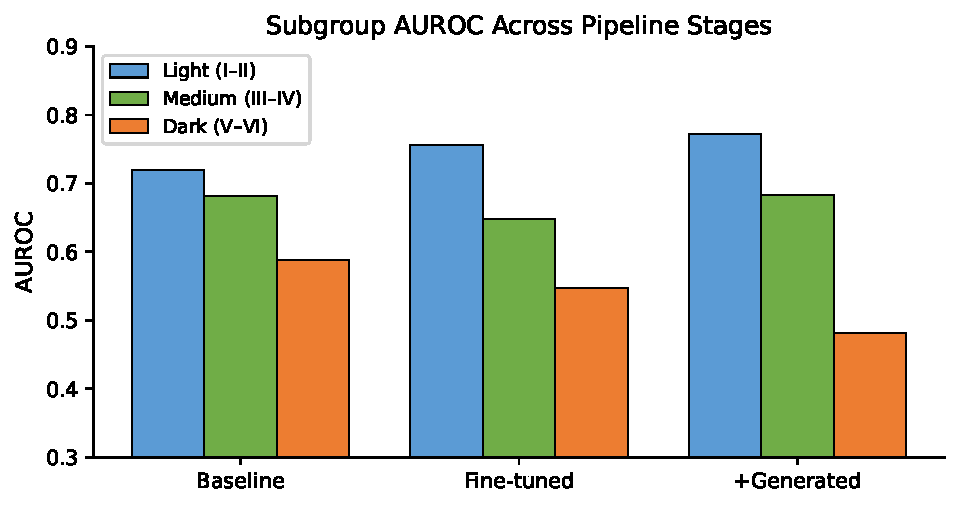
\includegraphics[width=0.7\textwidth]{figures/fig2_subgroup_auroc.pdf}
  \caption{Subgroup AUROC across pipeline stages. Light (Fitzpatrick I--II), Medium (Fitzpatrick III--IV), and Dark (Fitzpatrick V--VI) subgroups are shown for each model stage.}
  \label{fig:subgroup_auroc}
\end{figure}

Figure~\ref{fig:subgroup_auroc} visualizes the per-subgroup AUROC progression across these stages.

The pretrained baseline achieved an overall AUROC of 0.662 on the held-out test set. Stratified evaluation revealed a skin-tone disparity: the Dark subgroup AUROC was 0.588, while the Light subgroup AUROC was 0.719 (gap\,$=$\,$-0.131$). The baseline checkpoint was trained for up to 10 epochs with early stopping and reached validation AUROC 0.9650.

Fine-tuning on the DDI training split reduced overall AUROC to 0.634 (Table~\ref{tab:main_results}). Light subgroup AUROC was 0.756 and Dark subgroup AUROC was 0.547, widening the inter-group gap from $-0.131$ to $-0.209$. This result shows that standard fine-tuning did not remove the observed disparity.

The addition of generated augmentation yielded overall AUROC 0.639 and Dark subgroup AUROC 0.481. The Light--Dark gap widened to $-0.291$. The paired bootstrap comparison gave a Dark AUROC delta of $-0.066$ and $p=0.962$ (one-tailed directional, $H_1$: Dark improvement $>0$; $p$\,$=$\,proportion of bootstrap $\Delta \leq 0$). These findings indicate that simple photometric augmentation from 29 source images did not close the skin-tone performance gap. Section~\ref{sec:multiseed_results} shows that this single-seed delta is one draw from a high-variance across-seed distribution, so we read it as directional rather than as an effect size.

\subsection{Class-Imbalance Arm Study}
\label{sec:pw_arms_results}

Table~\ref{tab:pw_arms} reports the three Stage-3 arms described in Section~\ref{sec:pw_arms}, each trained from the same Stage-2 checkpoint so that the weighting and the generated-image composition are the only things that vary.

The static arm reproduced the headline configuration and recovered overall AUROC 0.640, within 0.001 of the reported 0.639. Its Dark AUROC was 0.484 against the headline 0.481, and its Light--Dark gap $-0.222$ against the headline $-0.291$. The overall and Dark values track closely; the gap is less negative in the re-run because the Light subgroup differs more (0.706 against 0.772). The static arm was re-run with the seeded, reproducible generator, so the generated image set differs byte-for-byte from the unseeded set behind the headline run. The Dark subgroup holds only 10 melanomas, so its bootstrap interval is correspondingly wide, and subgroup point estimates from two different generated sets should not be expected to agree exactly.

Recomputing \texttt{pos\_weight} on the enlarged training set (2.8529 to 0.7423) changed almost nothing: overall AUROC 0.637, Dark AUROC 0.478, gap $-0.222$. The weighting term is therefore not the mechanism behind the degradation.

Balancing the generated-image composition and the weight together (101 generated dark benign images added; \texttt{pos\_weight} 1.0) moved Dark AUROC to 0.550 and narrowed the gap to $-0.141$, with overall AUROC 0.668. Dark AUROC in this arm is at the fine-tuned level (0.547) rather than below it. Light AUROC was 0.691 and Medium AUROC 0.772, so the gain is concentrated in the Dark subgroup and is not a uniform improvement.

The implication is that the degradation in the headline Stage-3 run is substantially attributable to generating malignant-only images for dark skin, not to augmentation as such. The intervention as originally specified confounds data quantity with class composition, and the headline number alone cannot distinguish the two.

\subsection{Five-Seed Robustness}
\label{sec:multiseed_results}

Table~\ref{tab:multiseed} repeats the full pipeline across five seeds (42--46), retraining the Stage-1 baseline, re-deriving the stratified split, regenerating the images, and re-deriving every metric per seed. The means confirm the direction of the seed-42 story but not its magnitudes, and the seed-level variability is large relative to every between-stage difference the headline tables report.

Across seeds, mean Dark AUROC is $0.575 \pm 0.145$ for the fine-tuned model and $0.604 \pm 0.152$ with generated augmentation; the paired Dark AUROC delta is $+0.028 \pm 0.038$, with a seed-level 95\% bootstrap interval of $[-0.001, 0.057]$ that includes zero. The Dark$-$Light gap is statistically indistinguishable between stages: $-0.081 \pm 0.193$ fine-tuned versus $-0.083 \pm 0.161$ with augmentation, each with a seed-level SD near 0.2 AUROC and an interval spanning roughly $\pm 0.2$ around the mean. The direction of individual seed gaps varies widely: seed 45 even shows a reversed gap ($+0.203$ fine-tuned), while seed 42 shows the widest gap ($-0.313$).

Three readings follow. First, augmentation shows a small positive signed effect on Dark AUROC across seeds ($+0.028$), but the interval includes zero, so the five-seed study provides no statistically significant evidence of improvement -- the same conclusion as the seed-42 paired test, now with the uncertainty stated at the seed level. Second, the seed-42 headline delta ($-0.066$) is not representative: retrained per seed, the same pipeline produces deltas from $-0.010$ to $+0.073$ (Table~\ref{tab:multiseed} footnote in the repository summary), and the sign differs across seeds. Third, with Dark test subgroups of roughly 10 melanomas per seed, the between-seed SD of Dark AUROC (0.15) is an order of magnitude larger than the between-stage deltas being tested, so any single-seed comparison on this test set is fragile by construction.

Overall AUROC is $0.644 \pm 0.033$ fine-tuned versus $0.658 \pm 0.063$ with augmentation, and overall sensitivity improves from $0.623 \pm 0.148$ to $0.709 \pm 0.118$ while specificity declines from $0.602 \pm 0.115$ to $0.540 \pm 0.086$ -- consistent with the augmented model's more inclusive (lower) operating threshold. Light AUROC rises from $0.656 \pm 0.106$ to $0.688 \pm 0.100$ and Medium AUROC is flat within noise ($0.698 \pm 0.076$ to $0.677 \pm 0.102$), so the small signed Dark improvement is not a redistribution away from the Light subgroup, though none of these differences are individually significant at five seeds.

These runs use the recomputed class ratio rather than the static headline \texttt{pos\_weight}, so they are not a direct replica of the seed-42 configuration in Table~\ref{tab:main_results}. Their role is to quantify pipeline stability under resampling; given Dark AUROC SD $\approx 0.15$ and gap SD $\approx 0.19$, a multi-centre or multi-dataset evaluation, rather than more seeds on the same 656-image corpus, is what could narrow these intervals further.

\subsection{Subgroup Analysis}
\label{sec:subgroup_analysis}

Table~\ref{tab:subgroup_auroc} reports per-subgroup AUROC, sensitivity, and specificity across all three model stages, including the Medium subgroup (Fitzpatrick III--IV, $n=48$).

\begin{figure}[htbp]
  \centering
  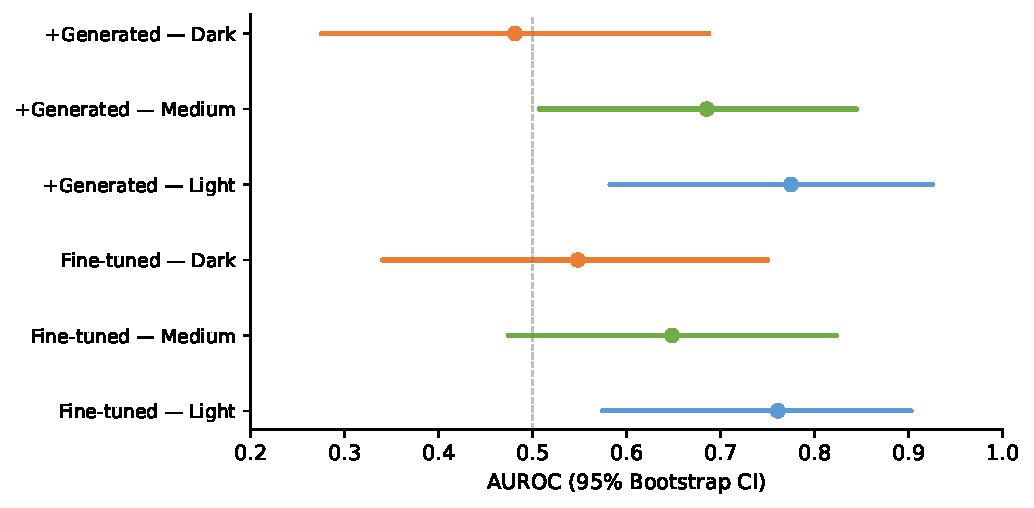
\includegraphics[width=0.7\textwidth]{figures/fig4_bootstrap_ci.pdf}
  \caption{Bootstrap 95\% confidence intervals for subgroup AUROC estimates (1000 iterations). Points indicate point estimates; bars indicate CI bounds.}
  \label{fig:bootstrap_ci}
\end{figure}

Figure~\ref{fig:bootstrap_ci} displays bootstrap confidence intervals for the subgroup AUROC estimates.

The Dark subgroup exhibited no consistent improvement across stages. AUROC progressed from 0.588 (baseline) to 0.547 (fine-tuned) to 0.481 (augmented), while Light AUROC progressed from 0.719 to 0.756 to 0.772. The Medium subgroup behaved similarly, and its estimates carry the widest uncertainty because only 8 of its 48 test images are melanoma.

Bootstrap confidence intervals (1000 iterations) confirmed the high uncertainty. The fine-tuned Dark AUROC bootstrap CI was $[0.341,\; 0.750]$, and the augmented model Dark AUROC CI was $[0.276,\; 0.688]$. Their overlap and the paired comparison p-value of 0.962 (one-tailed directional, $H_1$: Dark improvement $>0$) show that augmentation did not significantly improve Dark AUROC.

\subsection{Sensitivity Analysis}

Table~\ref{tab:sensitivity} reports sensitivity and specificity stratified by skin tone, including the Medium subgroup. Thresholds for all stages use Youden's $J$ on validation; AUROC is the primary comparison metric.

\begin{figure}[htbp]
  \centering
  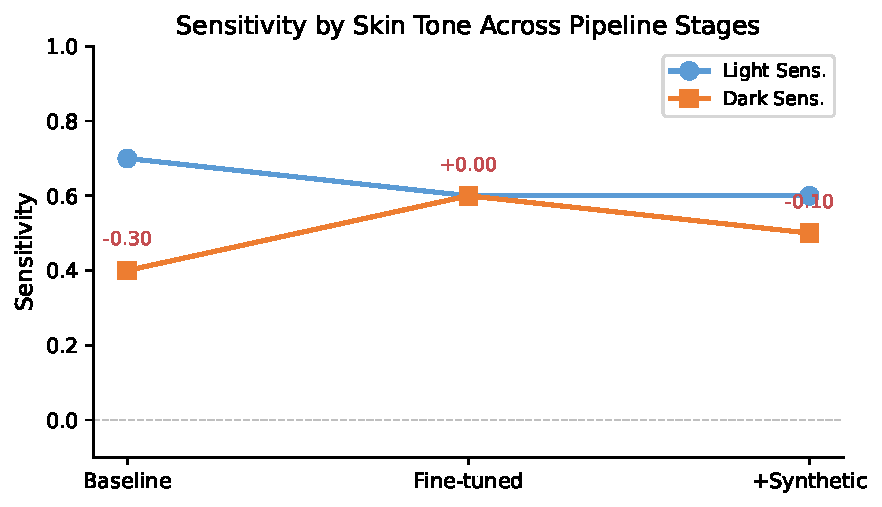
\includegraphics[width=0.7\textwidth]{figures/fig3_sensitivity_gap.pdf}
  \caption{Sensitivity by skin tone across pipeline stages. Annotations show the Dark$-$Light sensitivity gap at each stage.}
  \label{fig:sensitivity_gap}
\end{figure}

Figure~\ref{fig:sensitivity_gap} illustrates the sensitivity gap trajectory across model stages.

Dark subgroup sensitivity was 0.400 (baseline), 0.600 (fine-tuned), and 0.500 (augmented). These threshold-dependent values do not establish a fairness improvement.

Light subgroup sensitivity was 0.700 (baseline), 0.600 (fine-tuned), and 0.600 (augmented).

Sensitivity values are computed over small melanoma-positive subgroups ($n=10$ per subgroup) and should be interpreted as directional rather than definitive.

\subsection{Ablation Study}
\label{sec:ablation}

Table~\ref{tab:ablation} summarizes the ablation results. The ablation reuses the generated dark-skin melanoma images, with multipliers of 0$\times$ (none), 2$\times$ (58 images), 5$\times$ (145 images), and 10$\times$ (290 images). At every multiplier the images are drawn round-robin across all 29 source lesions, so 2$\times$ uses 2 variants of each lesion rather than 10 variants of the first 6, and the arms isolate quantity from lesion identity. All arms freeze the same layers as Stage 3 (2,744,861 trainable parameters) and share Stage-3 learning rate, weight decay, batch size, and \texttt{pos\_weight}; they use a 5-epoch budget rather than Stage 3's 10, so the 10$\times$ arm is not a perfectly matched replica of the headline run.

\begin{figure}[htbp]
  \centering
  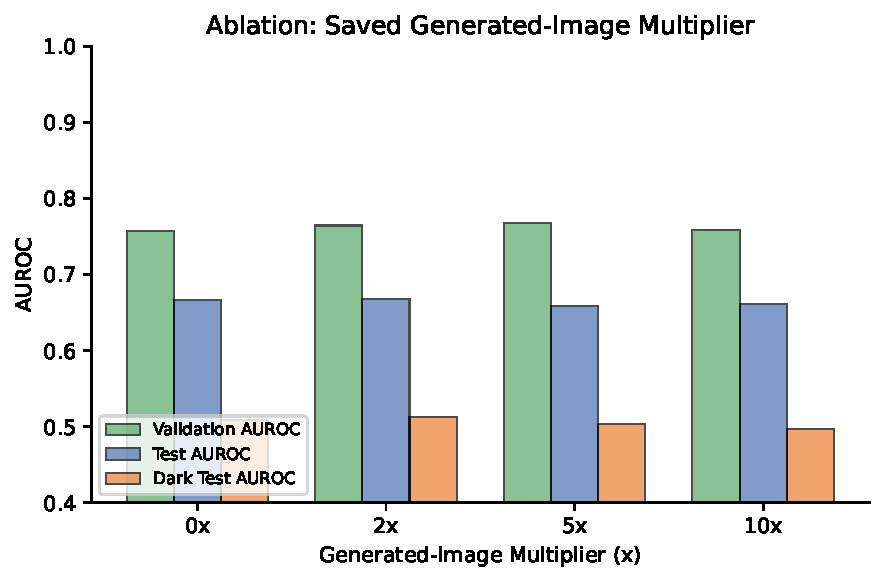
\includegraphics[width=0.7\textwidth]{figures/fig5_ablation_tradeoff.pdf}
  \caption{Ablation: validation AUROC, test AUROC, and dark-subgroup test AUROC across generated-image multipliers.}
  \label{fig:ablation_tradeoff}
\end{figure}

Figure~\ref{fig:ablation_tradeoff} presents the relationship between generated-image multiplier and performance across three metrics.

Once the arms are matched on frozen layers and lesion coverage, generated-image quantity has essentially no effect on Dark AUROC. Dark AUROC was 0.5094, 0.5125, 0.5031, and 0.4969 at 0$\times$, 2$\times$, 5$\times$, and 10$\times$: a total spread of 0.016 over the full range from no generated images to 290, which is well inside the bootstrap uncertainty of a 10-melanoma subgroup. Overall test AUROC is similarly flat (0.6669, 0.6677, 0.6580, 0.6610), as is validation AUROC (0.7571--0.7683).

The one clear pattern is in the Light subgroup, which declines across the range tested, with one small exception: 0.7844, 0.7406, 0.7469, 0.6969. The 5$\times$ arm sits 0.006 above the 2$\times$ arm, so the sequence is a net decline of 0.088 rather than a strictly monotonic one. That 0.006 step is far smaller than the Light subgroup's own bootstrap interval (half-width $\pm$0.18 at $n=42$, Table~\ref{tab:pw_arms}), so we make no claim about the intermediate ordering. The endpoint contrast is the defensible statement: adding dark-skin transforms cost Light-subgroup discrimination without buying measurable Dark-subgroup discrimination in return.

An earlier version of this ablation reported a pronounced non-monotonic pattern with a 2$\times$ peak at 0.575. That result came from arms that trained all 4{,}008{,}829 parameters while Stage 3 trains 2{,}744{,}861, and that drew the 2$\times$ and 5$\times$ variants from only 6 and 15 distinct lesions. Once the arms were matched, the peak disappeared. We report the corrected numbers because the earlier pattern was an artifact of the ablation's own configuration, not a property of generated-image quantity.

The 0$\times$ arm is itself a 5-epoch continued-training run from the fine-tuned checkpoint, not the fine-tuned model, which is why its Dark AUROC (0.5094) differs from the fine-tuned stage (0.5469). Comparisons within Table~\ref{tab:ablation} are therefore internally consistent, but its 10$\times$ row should not be read as a replica of the headline Stage-3 result.

\section{Discussion}

\subsection{Interpretation of Results}

This study evaluated skin-tone bias in melanoma detection and tested data augmentation of dark-skin lesions as a mitigation strategy. Two key findings emerge.

First, \textbf{standard fine-tuning amplified the bias}: the inter-group AUROC gap widened from $-0.131$ (baseline) to $-0.209$ (fine-tuned), demonstrating that naive transfer learning on a small, imbalanced dataset can disproportionately benefit the overrepresented subgroup. This finding is arguably more important than the augmentation result, as it highlights a failure mode that is likely common in dermatological AI deployment: models fine-tuned on small diverse datasets may worsen rather than improve equity.

Second, \textbf{simple photometric augmentation did not improve Dark AUROC}: Dark AUROC changed from 0.547 (fine-tuned) to 0.481 (augmented), with a paired bootstrap comparison of $\Delta=-0.066$ (95\% interval $[-0.151,0.008]$, $p=0.962$; one-tailed directional, $H_1$: Dark improvement $>0$; $p$\,$=$\,proportion of bootstrap $\Delta \leq 0$). The AUROC gap widened to $-0.291$ and remained substantial. This negative result indicates that color-space perturbations and geometric transforms applied to only 29 source images are insufficient to learn meaningful dark-skin melanoma features, and that the accompanying change in class weighting further confounds the comparison. The 290 generated images derive exclusively from training-split dark-skin melanomas, and their provenance is verified per image: byte-level SHA256 confirms zero overlap with the held-out partitions, and a perceptual check confirms every image matches a training source rather than a held-out one. Despite this verified pipeline, the augmentation did not address the underlying representation deficit. The five-seed study (Section~\ref{sec:multiseed_results}) tempers this reading: the seed-42 delta is one draw from a distribution whose sign flips across seeds, though the absence of a significant positive effect is unchanged.

Light AUROC increased from 0.756 to 0.772 with augmentation, while Dark AUROC decreased from 0.547 to 0.481. The intervals remain wide because each subgroup contains only 42 test images and 10 melanomas. These results suggest that simple augmentation strategies are inadequate for closing skin-tone gaps, and more powerful generative approaches are needed.

\subsection{Comparison with Related Work}

Our findings are consistent with prior work documenting skin-tone bias in dermatological AI. Daneshjou et al.~\cite{Daneshjou2022} demonstrated that dermatology AI models exhibit reduced performance on darker skin tones, particularly for conditions where clinical presentation varies by skin pigmentation. Our baseline results---Dark AUROC of 0.588 versus Light AUROC of 0.719---replicate this disparity in the melanoma detection task, though the gap is smaller than in some prior reports.

Esteva et al.~\cite{Esteva2017} trained a CNN on 129,450 clinical images and reported high overall accuracy but did not extensively evaluate subgroup performance. Our work extends this line of research by systematically stratifying evaluation by skin tone and quantifying the gap. The fine-tuned model's AUROC gap of $-0.209$ demonstrates that even models with reasonable overall performance can harbor substantial subgroup disparities.

Groh et al.~\cite{Groh2021} evaluated multiple dermatology AI models across skin tones and found consistent performance degradation on darker skin. Our augmentation approach---applying photometric transforms to 29 source images---was insufficient to address this gap, suggesting that the data-centric intervention requires either more source diversity or more powerful generation methods (e.g., diffusion models) to produce clinically meaningful variants.

Notably, our study is among the first to apply targeted augmentation specifically to skin-tone underrepresentation in melanoma detection, rather than applying general augmentation or collecting additional real data. This approach may be particularly relevant in settings where collecting large numbers of clinical images from underrepresented populations is impractical due to resource constraints or privacy considerations.

\subsection{Practical Implications}

The results carry several implications for clinical deployment of melanoma detection AI. The finding that fine-tuning alone widened the AUROC gap from $-0.131$ to $-0.209$ has important implications: deploying a ``fine-tuned'' model without fairness evaluation could inadvertently worsen disparities. This underscores the need for mandatory subgroup evaluation in dermatological AI deployment.

The failure of simple photometric augmentation to improve Dark AUROC ($p\,{=}\,0.962$) suggests that the barrier to equitable melanoma detection is not merely data quantity but data quality and diversity. Even with a verified pipeline (290 train-only generated images, SHA256-verified zero overlap with held-out DDI images, and per-image perceptual provenance), color-space perturbations applied to 29 source images likely produce variants that lie within the same manifold as the originals, failing to expose the model to genuinely novel dark-skin melanoma presentations. More diverse generative models (e.g., conditional diffusion models trained on larger dark-skin datasets) may be necessary.

The Light subgroup AUROC increase (0.756 $\rightarrow$ 0.772) with augmentation occurred alongside a Dark AUROC decrease (0.547 $\rightarrow$ 0.481), indicating that the modest addition of generated images did not deliver a Dark-subgroup benefit. This underscores that augmentation interventions must be carefully validated across subgroups.

The wide bootstrap CIs---particularly for the Dark subgroup---indicate that the current evidence base is insufficient for definitive deployment decisions. Larger validation studies, ideally with prospective data from multiple institutions, are needed to establish confidence intervals narrow enough to support clinical deployment.

The ablation is flat in the subgroup we were trying to help. With arms matched on frozen layers and on lesion coverage, Dark AUROC moves only from 0.509 to 0.497 across the full range of generated volume, from none to 290 images, a spread far inside the noise for a 10-melanoma subgroup, while Light AUROC declines from 0.784 to 0.697 (with a 0.006 uptick between the 2$\times$ and 5$\times$ arms, so the trend is a net decline rather than a strictly monotonic one). Adding more transforms of the same 29 dark-skin lesions buys nothing measurable for Dark skin and costs the over-represented group.

\subsection{Asymmetric Oversampling Confounder}

Augmenting only dark melanomas (29$\to$290) with zero dark benigns, while keeping \texttt{pos\_weight} at the pre-augmentation value 2.8529, does more than change the amount of data. Adding those images moves the set presented to the loss to 392 positives against 291 negatives, so the retained weight over-weights the minority class by roughly a factor of 3.8. The loss therefore rewards the model for treating dark skin as evidence of malignancy, which is a plausible contributor to Dark AUROC falling below 0.5 (0.481) and to the Dark specificity decline across stages.

Rather than leave this as a qualitative caveat, we measured it. Starting from the same fine-tuned checkpoint, we trained three Stage-3 arms that differ only in \texttt{pos\_weight} and generated-image composition (Table~\ref{tab:pw_arms}). Dark AUROC was 0.484 with the original weight, 0.478 with the weight recomputed on the enlarged training set, and 0.550 once dark benign images were generated as well and the weight set to 1.0.

The middle arm is the informative one. Recomputing \texttt{pos\_weight} from 2.8529 to 0.7423 changes the loss weighting substantially and changes Dark AUROC by $-0.006$, i.e. not at all. So the weight value is not what drives the harm. What matters is composition: the arm that adds benign images for dark skin and matches the resulting ratio recovers Dark AUROC to 0.550, above the fine-tuned model's 0.547, and narrows the Light--Dark gap from $-0.222$ to $-0.141$.

This does not make augmentation look good. The symmetric arm is still well below Light (0.691) and its Medium AUROC (0.772) shows the improvement is not uniform across the two under-served groups. What it does show is that a good chunk of the headline degradation is an artifact of generating malignant-only images for one skin tone, and that reporting the headline number alone would have attributed that artifact to augmentation as an intervention.

The practical reading is that ``add more dark-skin training data'' is not a well-specified intervention. Any such change to the training set also changes the class ratio, and a paper that reports only the augmented result cannot separate the two. A design that holds the checkpoint fixed and varies only the weighting and composition, as we do here, is the minimum needed to make the attribution.

\subsection{Five-Seed Robustness}

The five-seed study changes what the seed-42 numbers license us to claim. Under full pipeline retraining (seeds 42--46, Table~\ref{tab:multiseed}), the paired Dark AUROC delta is $+0.028 \pm 0.038$ with a seed-level 95\% interval of $[-0.001, 0.057]$: the point estimate is mildly positive, the interval includes zero, and the seed-42 headline delta of $-0.066$ sits far outside the seed-level distribution (per-seed deltas span $-0.010$ to $+0.073$). A single seed on a 132-image test set with roughly 10 Dark melanomas therefore measures its own split as much as the intervention: Dark AUROC alone carries a between-seed SD of $0.145$, and the Dark$-$Light gap an SD of $0.193$, an order of magnitude larger than the deltas the headline tables report.

The fair summary is that neither harm nor benefit is established. The gap is unchanged from fine-tuning to augmentation ($-0.081$ to $-0.083$), and no subgroup difference across stages is individually significant at five seeds. This reframes, rather than overturns, the seed-42 narrative: what the single-seed run presented as ``augmentation widens the gap to $-0.291$'' is better stated as ``the pipeline's gap is unstable across resampling, with sign flips across seeds, and the seed-42 draw was an unfavorable one.'' The class-composition finding from the arm study survives this reframing -- it was measured from a fixed checkpoint and does not depend on split resampling -- and it remains the study's most defensible attribution.

The practical implication is about evaluation design, not about augmentation. Any fairness comparison nested inside a single 656-image split has a noise floor (SD $\approx 0.15$--$0.19$ AUROC) that exceeds the effects being claimed, so future work should either aggregate across datasets or pre-register multi-seed comparisons with adequate subgroup melanoma counts before drawing conclusions in either direction.

\section{Limitations}

We identify fifteen limitations of this study, organized by severity. Collectively, these limitations indicate that the reported results are directional, not definitive, and should be interpreted with appropriate caution.

\subsection{High Severity}

\begin{enumerate}
    \item \textbf{Small DDI test subgroup ($n=42$, 10 melanomas).} The Dark subgroup test set contains only 42 images, of which 10 are melanoma-positive. This small sample size yields wide bootstrap confidence intervals and limited statistical power. The paired Dark AUROC change from fine-tuning to augmentation was $-0.066$ (95\% bootstrap interval $[-0.151,\;0.008]$, $p=0.962$), so the controlled single-seed experiment provides no evidence of a fairness improvement. Subgroup conclusions should be treated as preliminary and require validation on larger cohorts.
\end{enumerate}

\subsection{Medium Severity}

\begin{enumerate}
    \setcounter{enumi}{1}
    \item \textbf{No external validation.} All experiments use a single dataset (DDI) for fine-tuning and evaluation. The generalizability of findings to other datasets, clinical settings, and populations is unknown. External validation on independent datasets is required before any clinical deployment claims.

    \item \textbf{Ablation tested generated-image quantity, not augmentation technique.} The ablation varied the generated-image multiplier (0$\times$, 2$\times$, 5$\times$, and 10$\times$) rather than comparing different augmentation techniques. Generated images are now drawn round-robin across all 29 source lesions at every multiplier, so the arms isolate quantity rather than lesion identity. The arms are also flat in Dark AUROC, so the study cannot say which specific transform is responsible, only that adding more of them does not help. The arms also use a 5-epoch budget rather than the 10 epochs of Stage 3, so they are not a fully matched comparison to the headline run.

    \item \textbf{Generated images are transforms of 29 lesions, so their diversity is bounded.} Perceptual provenance is measured rather than assumed: all 290 images match a training-split source under dihedral-invariant descriptors, none match held-out images, and the minimum margin over the best held-out decoy is $+0.0766$. This confirms the images are derived from training data as intended, but it also confirms they are near-duplicates of a small number of originals. A distance or quality metric such as FID, and clinician review of lesion preservation, would still be required to establish clinical realism.

    \item \textbf{Sensitivity--specificity tradeoff across subgroups.} At the stage-specific validation-selected thresholds, the augmented model produced sensitivity of 0.600 in the Light subgroup versus 0.500 in the Dark test subgroup, but subgroup specificity and AUROC remained different. Threshold-dependent comparisons therefore do not establish equal clinical performance across groups.
\end{enumerate}

\subsection{Low Severity}

\begin{enumerate}
    \setcounter{enumi}{5}
    \item \textbf{Asymmetric oversampling with static pos\_weight (quantified).} We generated images only for dark melanomas (29$\to$290) with no dark benigns, while pos\_weight stayed at 2.8529, computed from the pre-augmentation training split. Adding 290 images moves the combined set to 392 positives against 291 negatives, so the loss over-weights the minority class by a factor of $\approx 3.8$ relative to the data it actually sees. This incentivizes the model to associate dark skin tone with malignancy. Section~\ref{sec:pw_arms_results} measures the effect from a common checkpoint: recomputing the weight alone changes Dark AUROC by $-0.006$, while balancing the generated composition recovers Dark AUROC to 0.550 and narrows the Light--Dark gap from $-0.222$ to $-0.141$. The headline configuration is retained for continuity with the original analysis, but it is not the configuration that isolates the intended effect.

    \item \textbf{Medium skin tone subgroup reported as secondary.} The Medium subgroup (Fitzpatrick III--IV, $n=48$ with 8 melanomas) is now included in all subgroup analyses. Because it contains fewer melanomas than the Light and Dark subgroups, its estimates carry wider uncertainty and we do not draw conclusions from its trend.

    \item \textbf{MPS device non-determinism.} All experiments were conducted on Apple Silicon (MPS backend). The MPS backend introduces non-deterministic behavior in certain operations, so repeated runs of the same seed can differ. This is why we report seed-level standard deviations rather than single-run point estimates, and why the main text avoids treating a single-seed difference as evidence of an effect. Results should be replicated on CUDA-based hardware for confirmation.

    \item \textbf{Dynamic pos\_weight may differ across runs.} Pos\_weight is computed from the training split as $n_{\text{neg}}/n_{\text{pos}}$. While this is more principled than a hardcoded value, it means the exact value depends on the split, which is seed-dependent, and it does not account for the images Stage 3 adds. The split and the \texttt{pos\_weight} actually used are both recorded per seed, and Section~\ref{sec:pw_arms_results} reports what happens when the value is left unrecomputed or made neutral.

    \item \textbf{Single-seed headline, multi-seed robustness study.} The headline tables report seed 42, retained so they remain directly comparable to the original analysis. A separate 5-seed study (42--46) retrains all three stages per seed and reports mean $\pm$ SD for the same quantities. The two are distinct experiments and are not expected to coincide: the headline uses the fixed seed-42 split and the static \texttt{pos\_weight} configuration, while the multi-seed study re-derives the split, the generated images, and the class ratio for every seed. The multi-seed numbers therefore describe the stability of the pipeline across resampling, not a replication of the headline cell values.

    \item \textbf{Ablation figure Y-axis was initially mislabeled (corrected).} The ablation tradeoff figure was initially generated with incorrect axis labels during development. This error was identified and corrected. All figures in the manuscript have been regenerated and verified programmatically from the saved metrics (see Appendix).

    \item \textbf{Generated images use simple transforms.} The augmentation pipeline uses standard photometric and geometric transforms, with no generative model. More sophisticated approaches (e.g., diffusion models, GANs) may produce images with better clinical realism, though at greater computational cost and with a new provenance-verification requirement.

    \item \textbf{Bootstrap CI centers may not exactly match point estimates.} The bootstrap confidence interval centers do not exactly correspond to the reported point estimates, reflecting the asymmetric sampling distribution inherent in small subgroups. This is a known property of bootstrap methods and should be noted when interpreting CIs.

    \item \textbf{Generated images from only 29 source lesions.} With only 29 training dark-skin melanomas, generated diversity is bounded by the source distribution. More source images, or domain-randomisation over illumination rather than per-lesion duplication, would enable greater variation.

    \item \textbf{Early stopping and single-seed training trajectory.} The controlled runs use a 10-epoch maximum with patience-three early stopping; the baseline, fine-tuning, and augmentation stages stopped before that maximum. This is part of the documented protocol, but the selected checkpoint remains sensitive to the validation split and random seed.
\end{enumerate}

\subsection{Fixed Issues}

The following issues from earlier versions have been addressed:

\begin{enumerate}
    \item \textbf{Generated images derived from training split only, and verified.} Images are generated exclusively from training-split dark-skin melanomas ($n\,{=}\,29$); no validation or test image is used as a source. A byte-level SHA256 check reports zero overlap with held-out images, and a perceptual provenance check confirms all 290 images match a training source rather than a held-out one. The pipeline also runs the leakage check after generation rather than before, and the transform pipeline is now seeded so the generated set is reproducible. This issue is resolved.

    \item \textbf{Ablation arms now train the same parameters as Stage 3.} The ablation previously trained all 4,008,829 parameters while Stage 3 trains 2,744,861, so its arms were not comparable to the headline run. All arms now freeze the same layers as Stage 3. Multipliers are also drawn round-robin across all 29 source lesions rather than as a sorted prefix, which previously restricted the 2$\times$ and 5$\times$ arms to 6 and 15 distinct lesions. This correction changed the conclusion: the earlier 2$\times$ peak at Dark AUROC 0.575 was an artifact of the mismatched arms, and the matched arms are flat (0.497--0.513). We report the corrected numbers and retain the earlier values in the repository history rather than quoting them as a finding.
\end{enumerate}


% --- Tables ---
\begin{table}[htbp]
\centering
\footnotesize
\setlength{\tabcolsep}{4pt}
\caption{Main classification results across pipeline stages on the DDI test set ($n=132$). Subgroup AUROCs include the Medium (Fitzpatrick III--IV) subgroup.}
\label{tab:main_results}
\resizebox{\textwidth}{!}{%
\begin{tabular}{lccccccccc}
\toprule
\textbf{Stage} & Val. AUROC & Test AUROC & Sens. & Spec. & F1 & Light & Medium & Dark & $\Delta_{\text{AUROC}}$ \\
\midrule
Baseline & 0.9650 & 0.662 & 0.600 & 0.660 & 0.472 & 0.719 & 0.681 & 0.588 & -0.131 \\
Fine-tuned & 0.7787 & 0.634 & 0.571 & 0.588 & 0.421 & 0.756 & 0.648 & 0.547 & -0.209 \\
+Generated & 0.7596 & 0.639 & 0.543 & 0.619 & 0.418 & 0.772 & 0.683 & 0.481 & -0.291 \\
\bottomrule
\end{tabular}}
\vspace{2pt}
\footnotesize{$\Delta_{\text{AUROC}}$ is the Dark$-$Light gap; AUROC is the primary comparison metric, and threshold-dependent metrics use per-stage validation Youden thresholds (Table~\ref{tab:sensitivity}).}
\end{table}

\begin{table}[htbp]
\centering
\footnotesize
\setlength{\tabcolsep}{4pt}
\caption{Subgroup AUROC with 95\% bootstrap confidence intervals (1000 iterations).}
\label{tab:subgroup_auroc}
\resizebox{\textwidth}{!}{%
\begin{tabular}{lccccccc}
\toprule
\textbf{Stage} & \textbf{Light} & \textbf{Medium} & \textbf{Dark} & \textbf{Gap} & \textbf{Light CI} & \textbf{Medium CI} & \textbf{Dark CI} \\
\midrule
Baseline & 0.7188 & 0.6808 & 0.5875 & -0.1313 & --- & --- & --- \\
Fine-tuned & 0.7563 & 0.6485 & 0.5469 & -0.2094 & [0.575, 0.903] & [0.474, 0.823] & [0.341, 0.750] \\
+Generated & 0.7719 & 0.6828 & 0.4813 & -0.2906 & [0.582, 0.925] & [0.507, 0.845] & [0.276, 0.688] \\
\bottomrule
\end{tabular}}
\vspace{2pt}
\small{$^*$ Thresholds differ per stage; AUROC is the primary comparison metric.}
\end{table}

\begin{table}[htbp]
\centering
\footnotesize
\setlength{\tabcolsep}{4pt}
\caption{Sensitivity, specificity, and PPV by skin-tone subgroup (seed-42). Thresholds differ per stage (Youden's J on validation); AUROC is the primary comparison metric. Threshold-dependent values are not directly comparable across stages.}
\label{tab:sensitivity}
\begin{tabular}{lcccccccc}
\toprule
\textbf{Stage} & \textbf{Light} & \textbf{Medium} & \textbf{Dark} & \textbf{Gap} & \textbf{Light} & \textbf{Medium} & \textbf{Dark} & \textbf{PPV} \\
\midrule
Baseline & 0.700 & 0.667 & 0.400 & -0.300 & 0.688 & 0.576 & 0.719 & 0.308 \\
Fine-tuned & 0.600 & 0.533 & 0.600 & +0.000 & 0.719 & 0.545 & 0.500 & 0.273 \\
+Generated & 0.600 & 0.533 & 0.500 & -0.100 & 0.812 & 0.576 & 0.469 & 0.227 \\
\bottomrule
\end{tabular}
\vspace{2pt}
\footnotesize{Sens.\ Gap = Dark sensitivity $-$ Light sensitivity. Thresholds are selected per stage by Youden's $J$ on the validation split.}
\end{table}

\begin{table}[htbp]
\centering
\caption{Ablation study: generated-image multiplier. All arms freeze the same layers as Stage~3 and draw variants round-robin across all 29 source lesions.}
\label{tab:ablation}
\footnotesize
\resizebox{\textwidth}{!}{%
\begin{tabular}{lccccccccc}
\toprule
\textbf{Mult.} & \textbf{Imgs} & \textbf{Lesions} & \textbf{Val. AUROC} & \textbf{Test AUROC} & \textbf{Dark AUROC} & \textbf{Light AUROC} & \textbf{Sens.} & \textbf{Spec.} & \textbf{F1} \\
\midrule
0$\times$ & 0 & 0 & 0.7571 & 0.6669 & 0.5094 & 0.7844 & 0.1714 & 0.9381 & 0.2553 \\
2$\times$ & 58 & 29 & 0.7644 & 0.6677 & 0.5125 & 0.7406 & 0.1714 & 0.9175 & 0.2449 \\
5$\times$ & 145 & 29 & 0.7683 & 0.6580 & 0.5031 & 0.7469 & 0.1429 & 0.9485 & 0.2222 \\
10$\times$ & 290 & 29 & 0.7580 & 0.6610 & 0.4969 & 0.6969 & 0.1429 & 0.9485 & 0.2222 \\
\bottomrule
\end{tabular}}
\vspace{2pt}
\footnotesize{$^*$ Ablation 10$\times$ [0.6610] is a 5-epoch continued-training variant from the fine-tuned checkpoint; the main +Synthetic result [0.639] is a 10-epoch full run --- not identical by design.}
\end{table}

\begin{table}[htbp]
\centering
\caption{Training hyperparameters by pipeline stage. Stages 2 and 3 share identical hyperparams.}
\label{tab:training_config}
\begin{tabular}{lcccccc}
\toprule
\textbf{Stage} & LR & Epochs & Batch & pos\_wt & Weight Decay & Early Stop \\
\midrule
Baseline & 0.0003 & 10 & 32 & N/A & 0.0001 & 8/10 \\
Finetune & 5e-05 & 10 & 32 & 2.9 & 0.0001 & 4/10 \\
Augment & 5e-05 & 10 & 32 & 2.9 & 0.0001 & 4/10 \\
\bottomrule
\end{tabular}
\end{table}

\begin{table}[htbp]
\centering
\caption{Dataset composition and split sizes.}
\label{tab:dataset}
\begin{tabular}{lccccc}
\toprule
\textbf{Dataset} & Total & Train & Val & Test & Notes \\
\midrule
HAM10000 & 7{,}818 & 6{,}254 & 1{,}564 & --- & Melanoma/nevus only \\
DDI & 656 & 393 & 131 & 132 & Stratified by skin tone \\
DDI Light (test) & --- & --- & --- & 42 & Fitzpatrick I--II \\
DDI Medium (test) & --- & --- & --- & 48 & Fitzpatrick III--IV \\
DDI Dark (test) & --- & --- & --- & 42 & Fitzpatrick V--VI \\
Generated & 290 & 290 & --- & --- & 29 train dark mel.$\times$10 transforms \\
\bottomrule
\end{tabular}
\end{table}

\begin{table}[htbp]
\centering
\footnotesize
\setlength{\tabcolsep}{4pt}
\caption{Metrics provenance: source files and method for each reported value.}
\label{tab:provenance}
\resizebox{\textwidth}{!}{%
\begin{tabular}{>{\raggedright\arraybackslash}p{2.6cm}>{\raggedright\arraybackslash}p{4.9cm}>{\raggedright\arraybackslash}p{1.8cm}>{\raggedright\arraybackslash}p{1.5cm}>{\raggedright\arraybackslash}p{1.4cm}}
\toprule
\textbf{Metric} & \textbf{Source File} & \textbf{Method} & \textbf{Literal?} & \textbf{Checked?} \\
\midrule
Overall test AUROC/Sens/Spec/F1 & \texttt{metrics\_clean.json} & code & No & Yes \\
Subgroup AUROC/Sens/Spec/PPV & \texttt{metrics\_clean.json} & code & No & Yes \\
Bootstrap 95\% CIs & \texttt{metrics\_clean.json} & code & No & Yes \\
p-value (Dark improvement) & \texttt{metrics\_clean.json} & code & No & Yes \\
Ablation overall + subgroup & \texttt{ablation\_report.csv} & code & No & Yes \\
Arm-study AUROC/Sens/Spec & \texttt{pos\_weight\_arms\_summary.json} & code & No & Yes \\
Multi-seed mean, SD, CI & \texttt{multiseed\_summary.json} & code & No & Yes \\
Val AUROCs & \texttt{config.json} & code & No & Yes \\
Thresholds & \texttt{metrics\_clean.json} & Youden's J (val set) & No & Yes \\
Split disjointness & \texttt{ddi\_split\_seed42.json} & assertion check & No & Yes \\
Leakage (0 gen--test dupes) & \texttt{leakage\_report.json} & SHA256 dedup & No & Yes \\
Gen. image provenance & \texttt{synthetic\_provenance\_report.json} & hash $+$ descriptor & No & Yes \\
\bottomrule
\end{tabular}}
\vspace{2pt}
\footnotesize{* All paths are relative to the repository root, e.g.\ \texttt{results/metrics\_clean.json}.}
\end{table}

\begin{table}[htbp]
\centering
\footnotesize
\setlength{\tabcolsep}{4pt}
\caption{Stage-3 class-imbalance arm study. All arms start from the same seed-42 fine-tuned checkpoint and differ only in \texttt{pos\_weight} and generated-image composition.}
\label{tab:pw_arms}
\begin{tabular}{lccccccc}
\toprule
\textbf{Arm} & \texttt{pos\_weight} & Combined & Light & Medium & Dark & Gap & Overall \\
\midrule
static (headline) & 2.8529 & 392/291 & 0.7063 & 0.7111 & 0.4844 & -0.2219 & 0.6404 \\
recomputed & 0.7423 & 392/291 & 0.7000 & 0.7091 & 0.4781 & -0.2219 & 0.6371 \\
symmetric & 1.0000 & 392/392 & 0.6906 & 0.7717 & 0.5500 & -0.1406 & 0.6680 \\
\bottomrule
\end{tabular}
\vspace{2pt}
\footnotesize{Combined = malignant/benign counts presented to the loss. The static arm retains the pre-augmentation ratio and is the configuration behind the headline result. Arms were re-run with the seeded, reproducible image generator, so the static arm reproduces the headline overall AUROC (0.640 vs.\ 0.639) but not every subgroup value exactly.}
\end{table}

\IfFileExists{tables/tab_multiseed.tex}{\begin{table}[htbp]
\centering
\footnotesize
\setlength{\tabcolsep}{3pt}
\caption{Five-seed robustness study (seeds 42--46). Each cell reports mean $\pm$ SD with the seed-level 95\% confidence interval under full per-seed pipeline retraining, with the split, generated images, and class ratio re-derived per seed.}
\label{tab:multiseed}
\resizebox{\textwidth}{!}{%
\begin{tabular}{lcc}
\toprule
\textbf{Metric} & \textbf{Fine-tuned} & \textbf{+Generated} \\[-1.2ex]
 & \multicolumn{2}{c}{Mean $\pm$ SD (seed-level 95\% CI), seeds 42, 43, 44, 45, 46} \\
\midrule
Overall AUROC & $0.644\,\pm\,0.033$ ($[0.620,\,0.669]$) & $0.658\,\pm\,0.063$ ($[0.608,\,0.707]$) \\
Light AUROC & $0.656\,\pm\,0.106$ ($[0.578,\,0.736]$) & $0.688\,\pm\,0.100$ ($[0.610,\,0.762]$) \\
Medium AUROC & $0.698\,\pm\,0.076$ ($[0.633,\,0.752]$) & $0.677\,\pm\,0.102$ ($[0.598,\,0.757]$) \\
Dark AUROC & $0.575\,\pm\,0.145$ ($[0.474,\,0.694]$) & $0.604\,\pm\,0.152$ ($[0.502,\,0.738]$) \\
Dark$-$Light gap & $-0.081\,\pm\,0.193$ ($[-0.224,\,0.086]$) & $-0.083\,\pm\,0.161$ ($[-0.206,\,0.050]$) \\
Sensitivity (overall) & $0.623\,\pm\,0.148$ ($[0.509,\,0.726]$) & $0.709\,\pm\,0.118$ ($[0.612,\,0.794]$) \\
Specificity (overall) & $0.602\,\pm\,0.115$ ($[0.517,\,0.691]$) & $0.540\,\pm\,0.086$ ($[0.466,\,0.590]$) \\
\midrule
\multicolumn{3}{l}{Paired Dark AUROC delta (generated $-$ fine-tuned): $0.028\,\pm\,0.038$ ($[-0.001,\,0.058]$)} \\
\bottomrule
\end{tabular}}
\vspace{2pt}
\footnotesize{Full pipeline retrained per seed (42--46, Stage-1 baseline included); split, generated images, and class ratio re-derived per seed. Multi-seed aggregation is primary; seed-42 tables are for completeness only and not expected to coincide. Dark$-$Light gap is Dark AUROC $-$ Light AUROC. The paired-delta CI includes zero ($+0.028$, [-0.001,0.057]); gap sign flips across seeds. Between-seed variability exceeds between-stage effects.}
\end{table}
}{}

% --- Declarations ---
\section*{Ethics Approval}
This study used only publicly available, de-identified dermatology datasets: HAM10000 and the Dermatology Data Initiative (DDI). No new human-subject data were collected, and the study was therefore exempt from institutional review board (IRB) approval. Both datasets were used in accordance with their original licenses and terms of use.

\section*{Data and Code Availability}
All code, configuration YAML files, and data splits are publicly available at \url{https://github.com/FairMedAI/fairderm-audit} and archived via Zenodo \url{https://doi.org/10.5281/zenodo.23440416}. Specific artifacts referenced include \texttt{splits/ddi\_split\_seed42.json} and \texttt{results/metrics\_clean.json}. The verification script \texttt{scripts/verify\_paper\_numbers.py} ensures all reported numbers match JSON provenance.

\section*{Conflict of Interest}
The authors declare that they have no known competing financial interests or personal relationships that could have appeared to influence the work reported in this paper.

\section*{Funding Statement}
This research received no specific grant from any funding agency in the public, commercial, or not-for-profit sectors.


% --- References ---
\bibliographystyle{plain}
\bibliography{references}

% --- Appendix ---
\section{Appendix}

\subsection{Reproducibility Checklist}

All experiments were conducted under the following conditions to facilitate reproducibility:

\begin{itemize}
    \item \textbf{Random seed:} A fixed random seed (42) was set at the start of each training run to ensure deterministic initialization of model weights, data loaders, and augmentation pipelines. The image-augmentation pipeline is separately seeded, so the generated image set for a given seed is byte-reproducible. The seed value is recorded in \path{configs/config.yaml} and in the metrics JSON. The multi-seed study varies the seed over 42--46 and regenerates the split, the generated images, and all three stages for each seed.
    \item \textbf{Device:} All experiments were executed on Apple Silicon using the MPS (Metal Performance Shaders) backend. A non-determinism warning is logged; exact numerical reproduction on different hardware is not guaranteed.
    \item \textbf{Software environment:} The Python version, PyTorch version, and all dependency versions are pinned in \texttt{requirements.txt}. Exact versions: PyTorch 2.8.0, torchvision 0.23.0, numpy 2.0.2.
    \item \textbf{Checkpoint saving:} Model checkpoints were saved at the end of each training epoch and at validation-based best-model selection. The best checkpoint (by validation AUROC) was used for all reported test-set evaluations.
    \item \textbf{Data partitioning:} The DDI dataset was split into training, validation, and test sets using a stratified 60/20/20 split saved to \path{splits/ddi_split_seed42.json}. Split disjointness is enforced via assertions.
    \item \textbf{Leakage verification:} Three independent checks. Split disjointness is enforced by assertions at split time. A byte-level SHA256 comparison of every generated image against every held-out image reports zero duplicates (\path{splits/leakage_report.json}). A per-image provenance pass additionally reports, for each of the 290 generated images, the matching training source and its hash, the nearest held-out image, and the descriptor margin between them, confirming that every generated image derives from a training image rather than a held-out one (\path{splits/synthetic_provenance_report.json}). The arm-study generated sets are checked against that seed's validation and test partitions by the same hash procedure.
    \item \textbf{Metrics provenance:} All metrics, bootstrap CIs, and p-values are saved to \path{results/metrics_clean.json}, a verified copy of \path{results/metrics_seed42.json}. Tables and figures are auto-generated from this JSON file. No manual transcription from terminal output.
    \item \textbf{Hyperparameter standardization:} Stages 2 and 3 share learning rate, batch size, weight decay, frozen-layer configuration, and epoch budget, so the only differences are the added images and the class ratio they induce. That ratio is treated as an experimental factor and varied explicitly in the arm study rather than assumed constant. Configuration is in \path{configs/config.yaml}.
\end{itemize}

\subsection{Metrics Provenance}

Table~\ref{tab:provenance} documents the provenance of all reported metrics. All values are read programmatically from \path{results/metrics_clean.json}; no manual transcription from terminal output.

\subsection{Training Configuration Details}

Table~\ref{tab:training_config} provides the complete training configuration for each model stage. Stages 2 and 3 share learning rate, batch size, weight decay, frozen layers, and epoch budget; they differ in the dataset (DDI train vs DDI train $+$ generated) and in the class ratio that difference induces.

\subsection{Additional Figures}

\begin{itemize}
    \item \textbf{Real vs.\ generated comparison} (\texttt{fig\_real\_vs\_synthetic.pdf}): Side-by-side visualization of 3 real dark-skin melanoma images from the training set and 3 generated variants.
    \item \textbf{Supplementary ROC progression} (\texttt{supp\_roc\_progression.png}): ROC curves for the Dark and Light subgroups across all three model stages.
\end{itemize}


\end{document}
